\documentclass[conference]{IEEEtran}
\IEEEoverridecommandlockouts
% The preceding line is only needed to identify funding in the first footnote. If that is unneeded, please comment it out.
 \usepackage[table,xcdraw]{xcolor}
\usepackage{cite}
\usepackage{amsmath,amssymb,amsfonts}
\usepackage{algorithmic}
\usepackage{graphicx}
\usepackage{textcomp}
\usepackage{xcolor}
\usepackage{hyperref}
\usepackage{mathtools}
\usepackage{comment}
\DeclarePairedDelimiter\ceil{\lceil}{\rceil}
\DeclarePairedDelimiter\floor{\lfloor}{\rfloor}

\def\BibTeX{{\rm B\kern-.05em{\sc i\kern-.025em b}\kern-.08em
    T\kern-.1667em\lower.7ex\hbox{E}\kern-.125emX}}
    
\begin{document}



\title{Applied Deep Learning Coursework}

\author{\IEEEauthorblockN{Kheeran Naidu}
\IEEEauthorblockA{\textit{Department of Computer Science} \\
\textit{University of Bristol}\\
kn16063@bristol.ac.uk}
\and
\IEEEauthorblockN{Adam Pluck}
\IEEEauthorblockA{\textit{Department of Computer Science} \\
\textit{University of Bristol}\\
ap16894@bristol.ac.uk}
\and
\IEEEauthorblockN{Farrel Zulkarnaen}
\IEEEauthorblockA{\textit{Department of Engineering Mathematics} \\
\textit{University of Bristol}\\
fz16336@bristol.ac.uk}

}

\maketitle

% --------------------------------------------------------------------------------
% \begin{abstract}
% This document is a model and instructions for \LaTeX.
% This and the IEEEtran.cls file define the components of your paper [title, text, heads, etc.]. *CRITICAL: Do Not Use Symbols, Special Characters, Footnotes, 
% or Math in Paper Title or Abstract.
% \end{abstract}
% \begin{IEEEkeywords}
% Keywords
% \end{IEEEkeywords}

% --------------------------------------------------------------------------------
\section{Introduction}
Definition of the problem addressed by the paper Su et al

% --------------------------------------------------------------------------------
\section{Related Work}
\textbf{A summary of published papers attempting to address the same problem (up to 3 works). These could be from the references of the paper itself, or otherwise.}\\

Within the domain of sound classification, and more specifically environmental sound, a wide scope of methods have been explored, ranging from complex to simplistic.

Piczak et al. \cite{piczak} first attempted to capitalise on the success of convolutional neural networks in other domains. Their architecture consisted of two convolutional layers each with max-pooling leading into two fully connected layers. All bar the 2nd convolutional layer were equipped with dropout. They achieved an accuracy of 73.1\% (LP) when trained and evaluated on a common dataset for this problem (\textit{UrbanSound8K}).

This success set off a flurry of CNN related methods, with the majority focusing on features. Similarly used by Su et al., Meyer et al. \cite{meyer} successfully incorporated the mel-spectrogram (log for Su) as a feature of the CNN. This was done by using mel-spectrogram as the transformer of the raw audio signal into a time-frequency representation (referred to as the ``front-end'').

Other methods took a different approach, attempting to negate the ill-effects of CNNs arising an ESC setting. Chen at al. \cite{chen} saw the negative effects of information loss as a result of max-pooling and so implemented dilated convolution: dilating or contracting convolutions (increasing/decreasing the receptive field) for the higher layers. This allows for an equal amount of a parameters compared to a conventional model, but with much lower levels of information loss. The success of this is clear. A dilation based model achieved an accuracy of 78\%, beating Piczak et al.'s model by a good margin. 
This model was also trained and evaluated on (\textit{UrbanSound8K}) which will now be explained.



\begin{comment}

WaveNet - Of two parts: multi-scale convolution operation and feature fusion.

Multi-scale convolution operation:

Pass waveform through a time-domain convolution with a fixed size, pool creating invariance to phase shifts and then down sample. As the name suggests, this is done multiple times for three different scales, better balancing the trade off between frequency resolution and time resolution.


Proposed in 2018, it is a multi-scale convolution operation, that gets a better audio representation by improving the frequency resolution and learning filters cross all frequency area.

Multiscale convolutional neural network that extracts features by filter banks (????) at multiple different scales and then fuse the log-mel features in the same model.

This is 3\% more accurate within classification problems when compared to a model using the same filters number (uses only waveform as input)

Feature fusion

\end{comment}
% --------------------------------------------------------------------------------
\section{Dataset} \label{section:dataset}
\textbf{A description of the dataset used, training/test split size, labels and file formats.}\\

The widely used UrbanSound8k data set is comprised of 8732 audio clips, each labelled as one of the 10 following classes: air conditioner (ac), car horn (ch), children playing (cp), dog bark (db), drilling (dr), engine idling (ei),gunshot (gs), jackhammer (jh), siren (si) and street music (sm). In our adaptation of this we divide the clips into multiple parts, treating each part as an independent training sample. For the validation aspect of the data set, we test on each part and then recombine to assess the final score and ultimately final classification. The overall proportion of test samples was just below 10\% (50569:5395). 

To neatly organise the divisions and other key features, the structure of the data set is simply a list of dictionaries with multiple keys (filename, class, classId, features). By making use of a dataloader we un-pickled (de-serialized) the data, ready to be modified into the two distinct inputs for each ``stream'' of the CNN. 



\begin{comment}

The train and test sets of the dataset are saved in UrbanSound8K_train.pkl, and UrbanSound8K_test.pkl.

The dataset is structured as a list of dictionaries. Each dict in the list corresponds to a different audio segment from an audio file. The dicts contain the following keys:

· filename: contains a unique name of the audio file. This is useful for matching audio segments to the audio file that they are coming from, and compute global scores by averaging the segments scores that have the same filename
· class: class name
· classID: class number [0…9]
· features: all the features to be used for training. This is a dictionary which contains: logmelspec, mfcc, chroma, spectral_contrast, Tonnetz


Pg 7 Experiment and Analysis:

\end{comment}
% --------------------------------------------------------------------------------
\section{Input}
\textbf{Explain the LMC and MC inputs used. Give 1-2 examples visually from your data, by plotting these as images. Do not use the figure from the original paper. }\\

\begin{figure}[h]
    \centering
    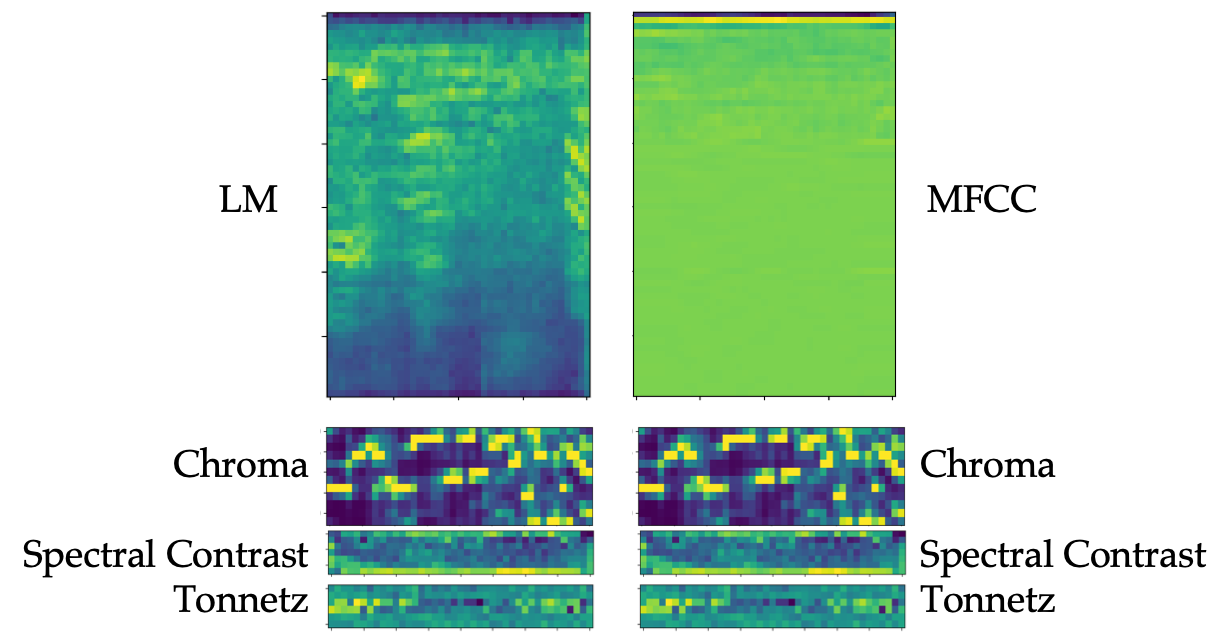
\includegraphics[width=0.5\textwidth]{images/input.png}
    \caption{Both inputs for a single data point: LMC (left) and MFCC (right)}
    \label{fig:inputSpectrogram}
\end{figure}{}

Given the two stream nature of the model, there are two different inputs to be prepared: LMC and MC. Although they share both three key auditory features (chroma, spectral contrast and tonnetz) and the method of combination (i.e concatenation), they are still distinctly different. LMC is the combination of the three shared features (referred to as CST) and the log-mel spectrogram (LM). Whereas, MC, is a combination of the CST and Mel Frequency Cepstral Coefficients (MFCC). A log mel-spectrogram is a representation of frequencies with the mel-scale (a logarithmic transformation) applied. MFCC, in contrast, is a representation of the envelope of short term power spectrum of the audioclips - typically used to represent phonemes of speech. \href{http://practicalcryptography.com/miscellaneous/machine-learning/guide-mel-frequency-cepstral-coefficients-mfccs/}{ref}



% --------------------------------------------------------------------------------
\section{Architecture (Su et Al)} \label{section:Architecture}
\textbf{Summarise the 4-conv architecture’s details, in writing, through a table or a diagram (only one of these). Detail your findings of where the paper’s inconsistencies are, and how you went around resolving these.} 


\subsection{Inconsistencies/errors:}



Confusion with stride length maybe?

\href{https://machinelearningmastery.com/padding-and-stride-for-convolutional-neural-networks/}{useful link for padding and stride}
In figure 4 conv1 to conv 2 has same dimensions so surely 2x2 stride mentioned in 3.2 doesn't make sense?
conv2 to conv3 has 2x2 max pooling, halving dimensions which makes sense with architecture
3.2 again mentions a stride of 2x2 conv3 to conv4 but dimensions stay the same?

Either stride is wrong with padding 1 or stride is correct but padding is 2

i.e stride 2x2 halves it then the padding doubles it keeping the dimensions the same after conv
or we have stride of 1 which doesn't have keeping the dimensions the same after conv

note stride of 2x2 in conv4 could be correct as input is 21x43 in figure 4, and at bottom of page 7 it says ``features with size of 11x22 are derived from the last hidden layer and feed to the fully-connected layer''

In figure 2, they don't specify the dimensions of the first bit

For a matrix of size $n\times m$ the output size after applying a kernel of size $f_{n}\times f_{m}$ would be:

\begin{equation}
    n_{output} = \floor{\frac{n+2p-f_{n}}{s} + 1}
\end{equation}

\begin{equation}
    m_{output} = \floor{\frac{m+2p-f_{m}}{s} + 1}
\end{equation}

where $p$ is the number of padding and $s$ is the number of stride
\\

Using the equations above we can deduce that the correct value for padding and the stride in order to achieved the specified output shape given in the paper. Using this formula as well we can further conclude that inconsistency found in the original paper was either that of a misspecified stride or padding value. In the paper it was stated that they used a stride of 2, but this will not lead the correctly specified output shape for the next layer. To retcon this mistake we believe that $p=1$ and $s=1$. Or alternative if we believe that the stride value is correct, i.e. $s=2$, as it is in the paper, then the required padding value would be 21 across and 43 down.




% --------------------------------------------------------------------------------
\section{Implementation Details}
\textbf{Summary of the steps you have undertaken to replicate the results, train the data and obtain the results, including any decisions you needed to make along the way. Do not include any pieces of code, but you can include pseudo-codes if needed. }

The implementation of the replicated results was based on the skeleton code provided for the course lab work.

The implementation uses 3 main classes; the CNN class, the Trainer class and the UrbanSound8KDataset class. The CNN class defines the architecture described in section \ref{section:Architecture}. The Trainer class contains the actions taken at each of the epochs associated with training. Finally, the UrbanSound8KDataset class provides the data in a standard format for PyTorch's DataLoader. 

Based on the format of the data, described in section \ref{section:dataset}, we used PyTorch's 2D Dropout, BatchNorm, MaxPool and Conv functions to define the neural network.

Replicating the results required careful fine tuning of the hyperparameters not defined in the given paper. These included the weight decay associated with the L2 regularisation, catering for the unbalanced class distribution of the data set and the type of variant of the SGD optimiser. The final replication results used the SGD optimiser with L2 regularisation and a weight decay of $10^{-2}$. 

% --------------------------------------------------------------------------------
\section{Replicating Quantitative Results}
\textbf{Your table 2 replication results. }

% Please add the following required packages to your document preamble:
% \usepackage[table,xcdraw]{xcolor}
% If you use beamer only pass "xcolor=table" option, i.e. \documentclass[xcolor=table]{beamer}
\begin{table}[h]
\begin{tabular}{|l|l|l|l|l|}
\hline
\textbf{Class} & \textbf{LMC (LMCNet)} & \textbf{MC (MCNet)} & \textbf{MLMC} & \textbf{TSCNN} \\ \hline
ac             & 48.3                  & 78.0                & 55.1          & 56.8           \\ \hline
ch             & 97.4                  & 71.1                & 92.1          & 94.7           \\ \hline
cp             & 74.4                  & 84.6                & 94.0          & 82.1           \\ \hline
db             & 68.1                  & 54.0                & 71.7          & 74.3           \\ \hline
dr             & 75.4                  & 80.5                & 81.4          & 78.0           \\ \hline
ei             & 60.5                  & 75.2                & 65.1          & 73.4           \\ \hline
gs             & 100.0                 & 100.0               & 97.1          & 97.1           \\ \hline
jh             & 99.1                  & 95.6                & 94.7          & 97.3           \\ \hline
si             & 50.0                  & 54.1                & 57.1          & 58.2           \\ \hline
sm             & 80.5                  & 84.7                & 74.6          & 78.8           \\ \hline
\rowcolor[HTML]{C0C0C0} 
\textbf{Avg.}  & \textbf{75.4}         & \textbf{77.8}       & \textbf{78.3} & \textbf{79.1}  \\ \hline
\end{tabular}
\\
\caption{Replicated class-wise accuracy of four models with four-layer CNN evaluated on our split of UrbanSound8K.}
\end{table}

% --------------------------------------------------------------------------------
\section{Training Curves}
\textbf{Include your training/test loss (and avg accuracy) curves for your models, and comment on any over fitting in your training. The tables here should correspond to the same run as those in the reported table (Section H). These curves could be directly retrieved from Tensorboard. }

\subsection{LMC}

\begin{figure}[h]
    \centering
    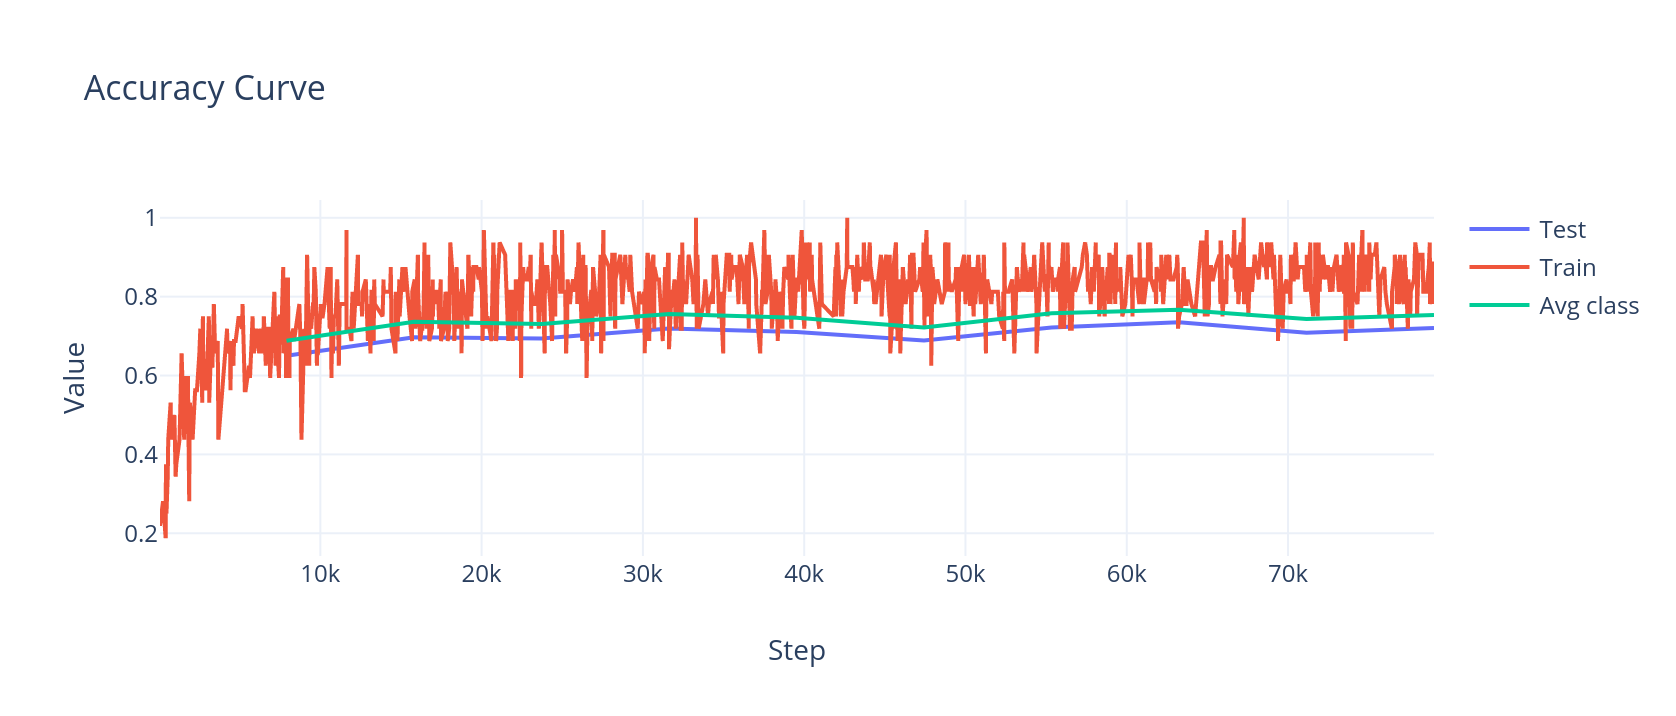
\includegraphics[width=0.5\textwidth]{images/LMC_accuracy.png}
    \caption{LMC Accuracy Curve}
    \label{fig:LMC_accuracy}
\end{figure}{}

\begin{figure}[h]
    \centering
    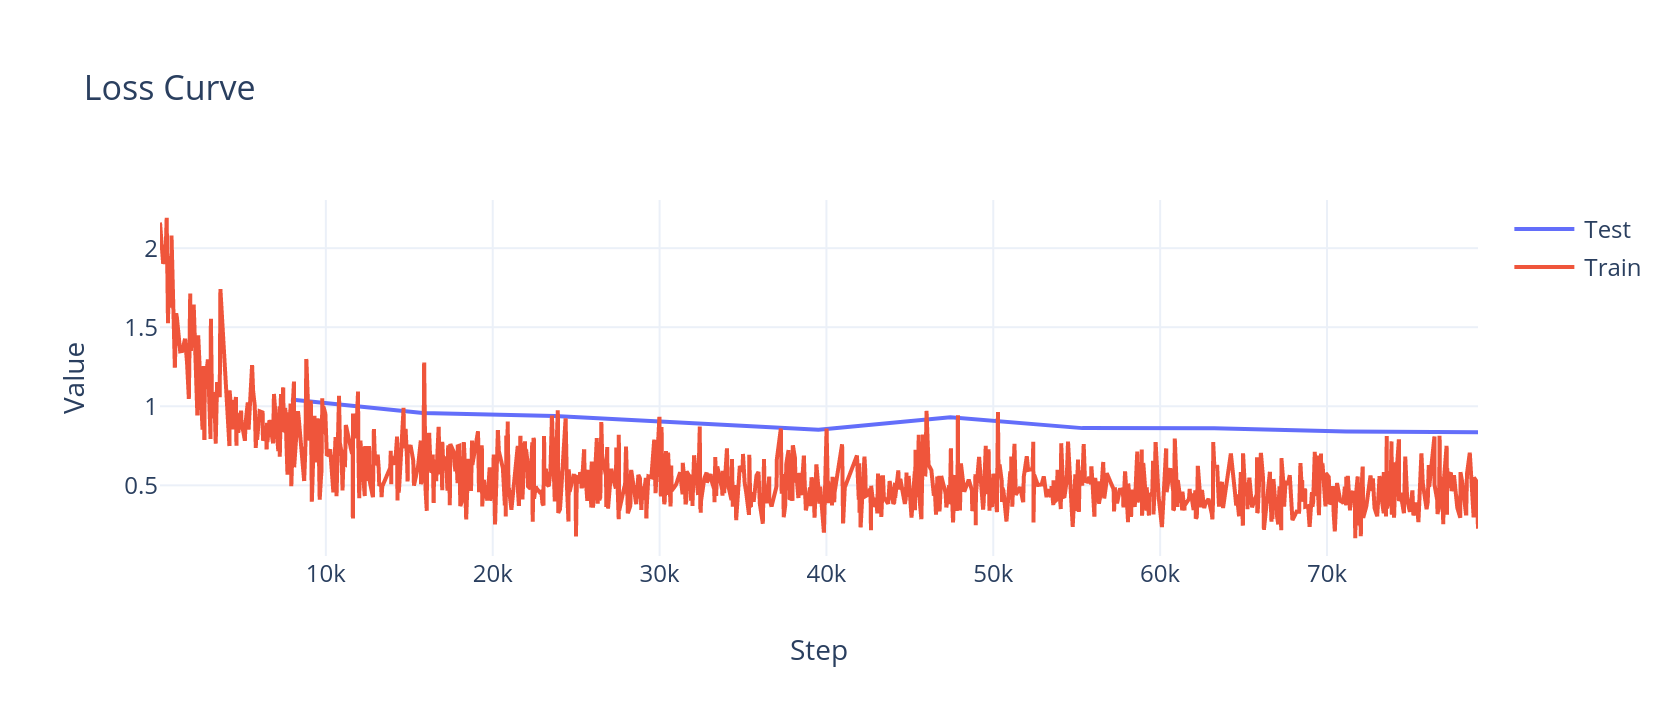
\includegraphics[width=0.5\textwidth]{images/LMC_loss.png}
    \caption{LMC Loss Curve}
    \label{fig:LMC_loss}
\end{figure}{}

\subsection{MC}

\begin{figure}[h]
    \centering
    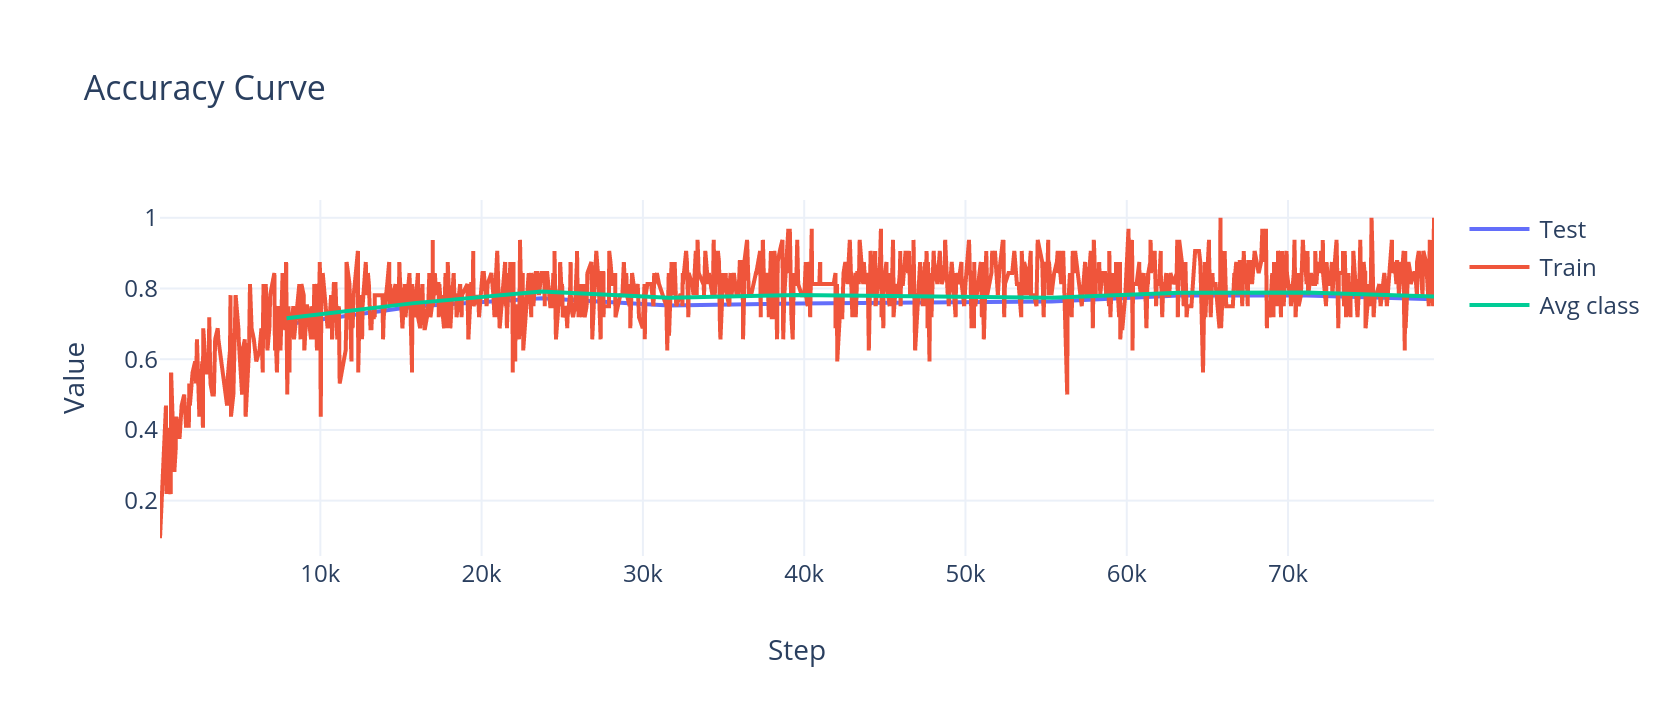
\includegraphics[width=0.5\textwidth]{images/MC_accuracy.png}
    \caption{MC Accuracy Curve}
    \label{fig:MC_accuracy}
\end{figure}{}

\begin{figure}[h]
    \centering
    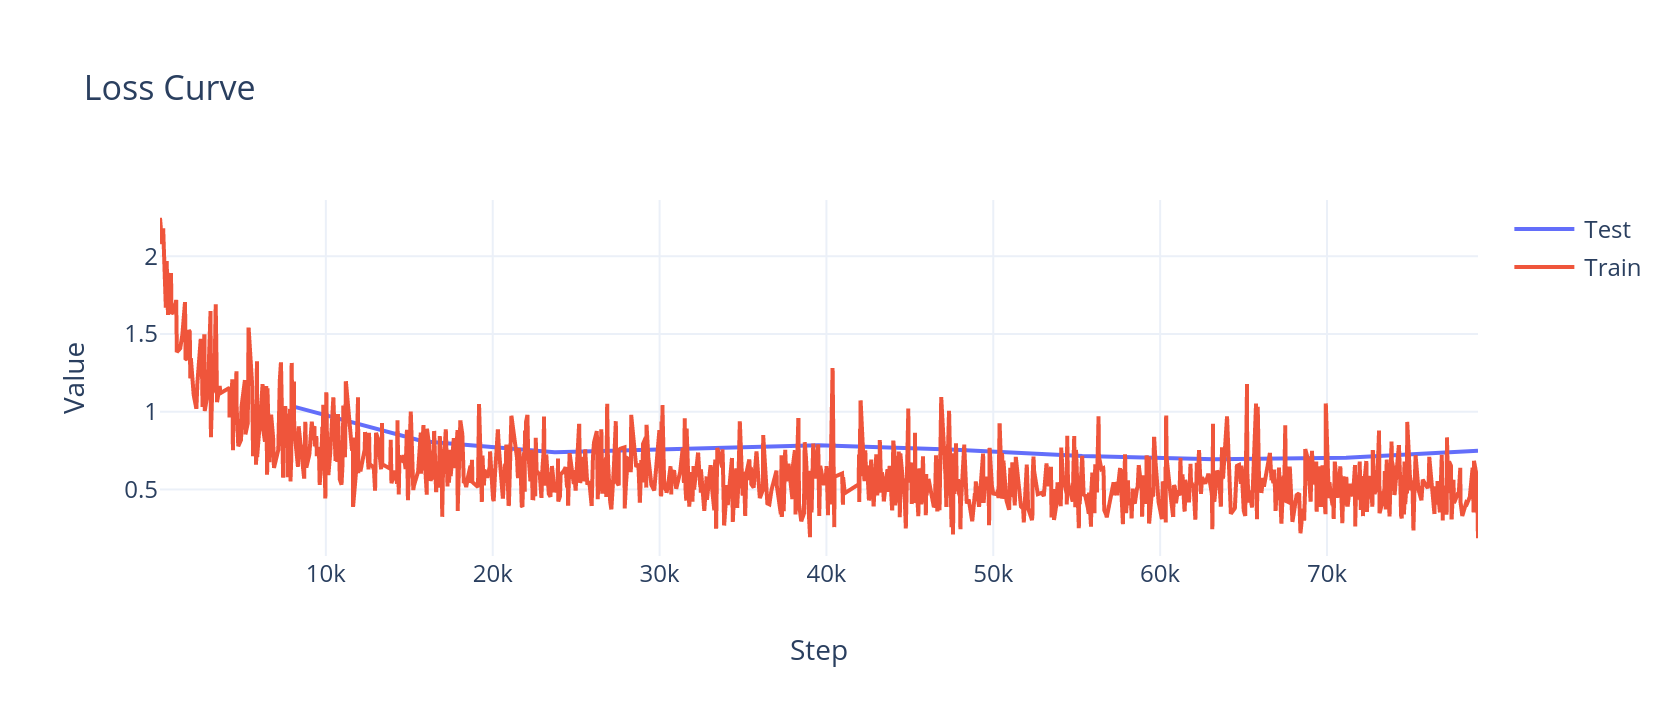
\includegraphics[width=0.5\textwidth]{images/MC_loss.png}
    \caption{MC Loss Curve}
    \label{fig:MC_loss}
\end{figure}{}

\subsection{MLMC}

\begin{figure}[h]
    \centering
    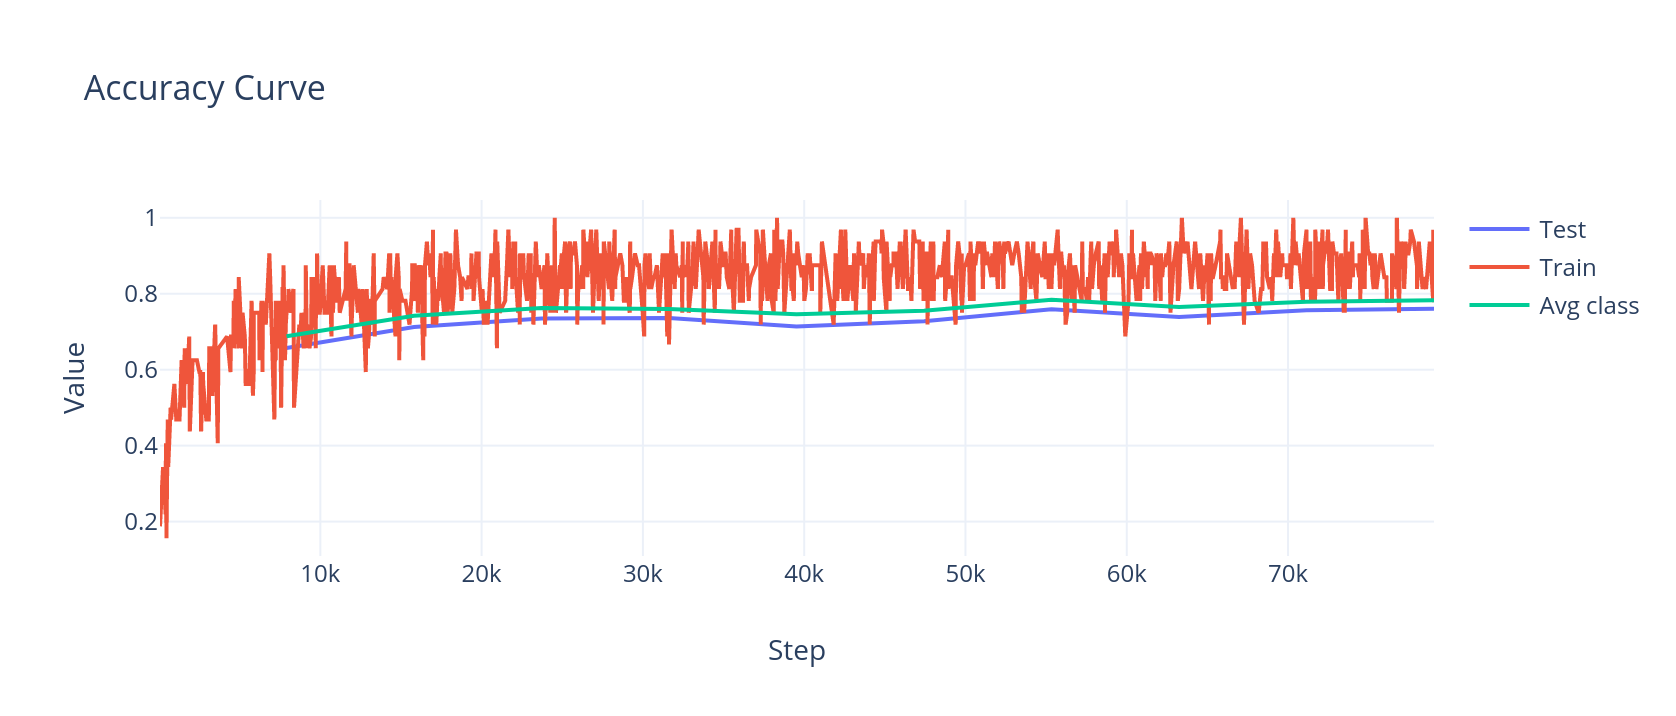
\includegraphics[width=0.5\textwidth]{images/MLMC_accuracy.png}
    \caption{MLMC Accuracy Curve}
    \label{fig:MLMC_accuracy}
\end{figure}{}

\begin{figure}[h]
    \centering
    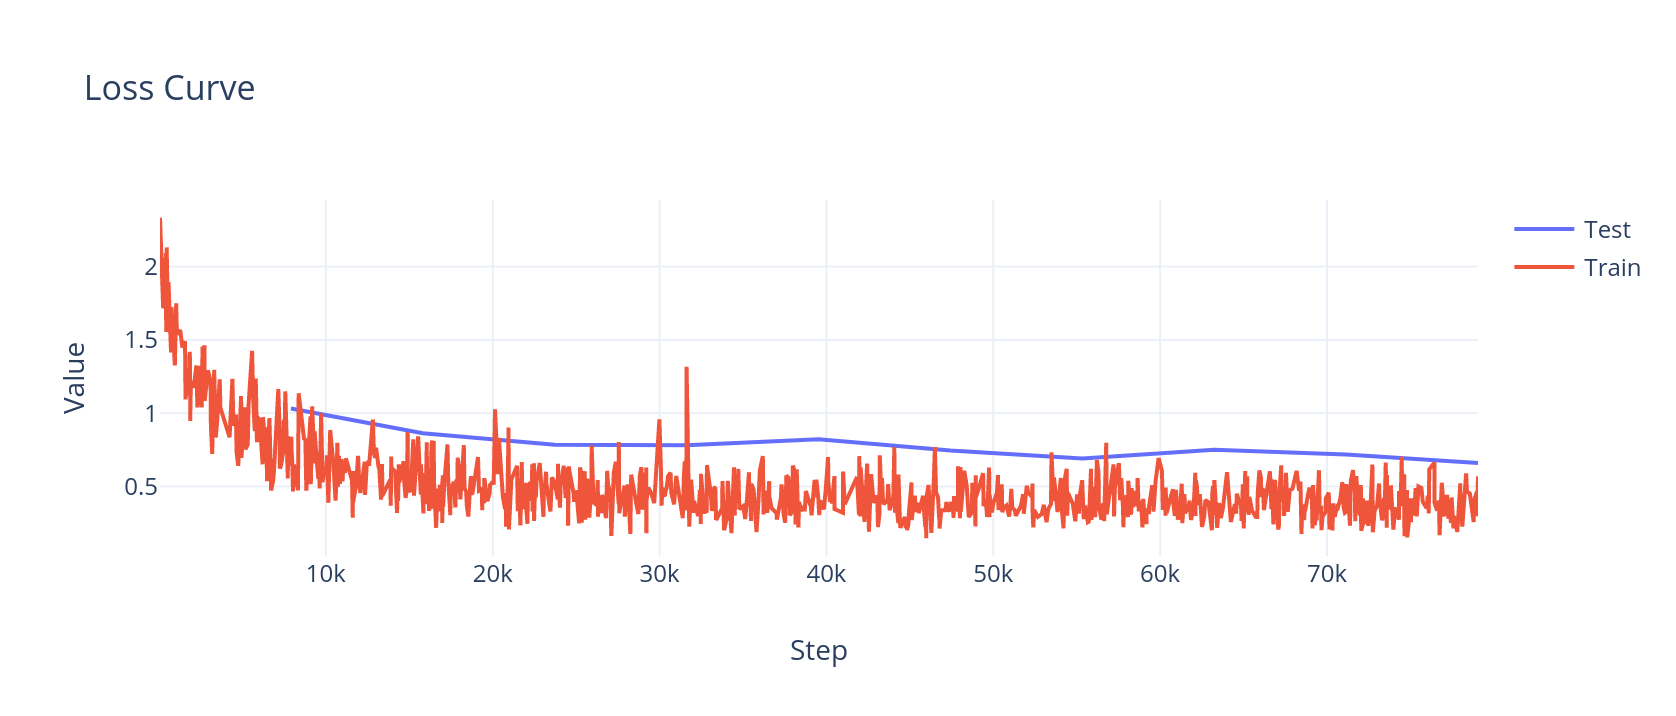
\includegraphics[width=0.5\textwidth]{images/MLMC_loss.png}
    \caption{MLMC Loss Curve}
    \label{fig:MLMC_loss}
\end{figure}{}

\subsection{TSCNN}

\begin{figure}[h]
    \centering
    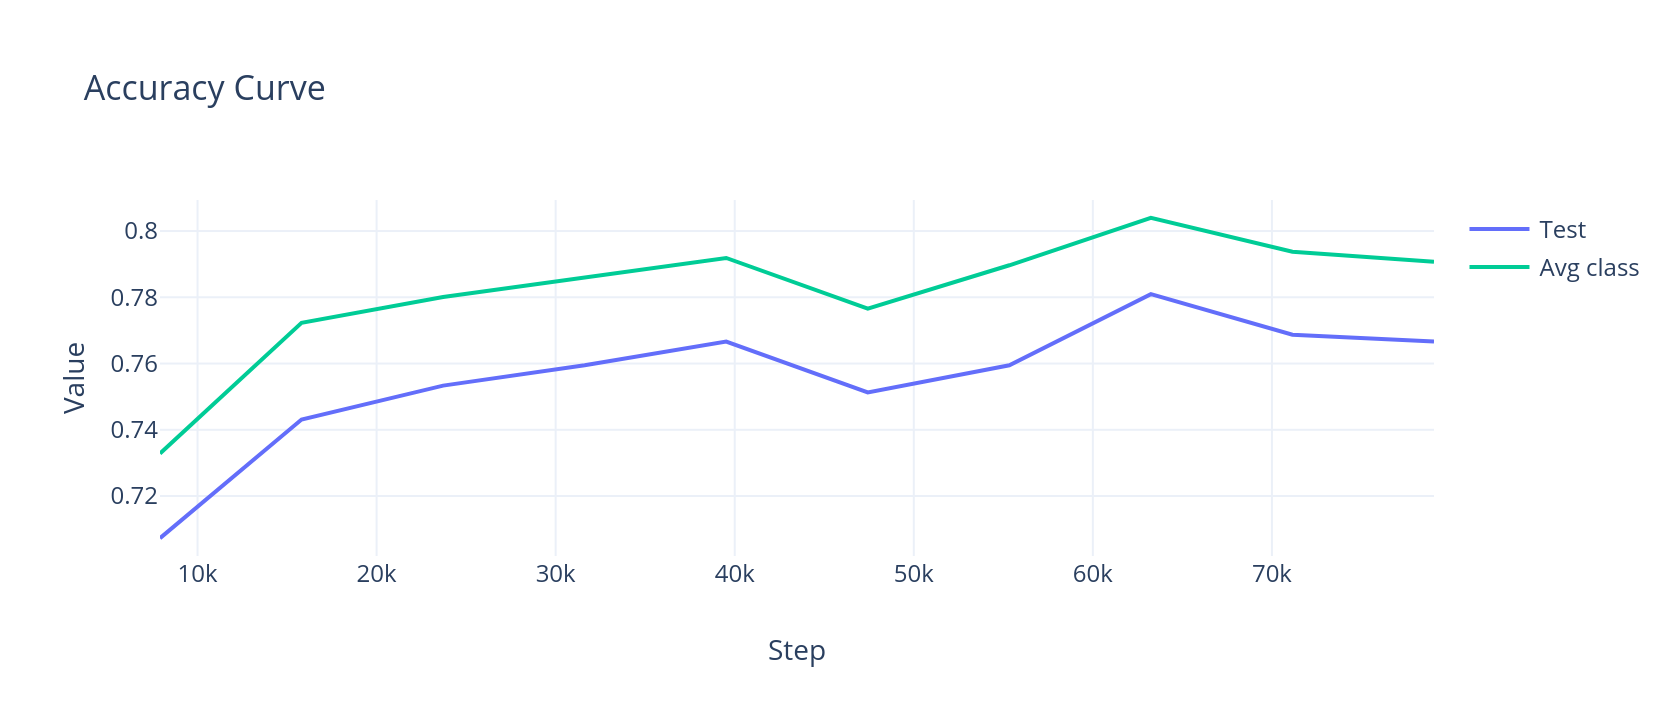
\includegraphics[width=0.5\textwidth]{images/TSCNN_accuracy.png}
    \caption{TSCNN Accuracy Curve}
    \label{fig:TSCNN_accuracy}
\end{figure}{}

\begin{figure}[h]
    \centering
    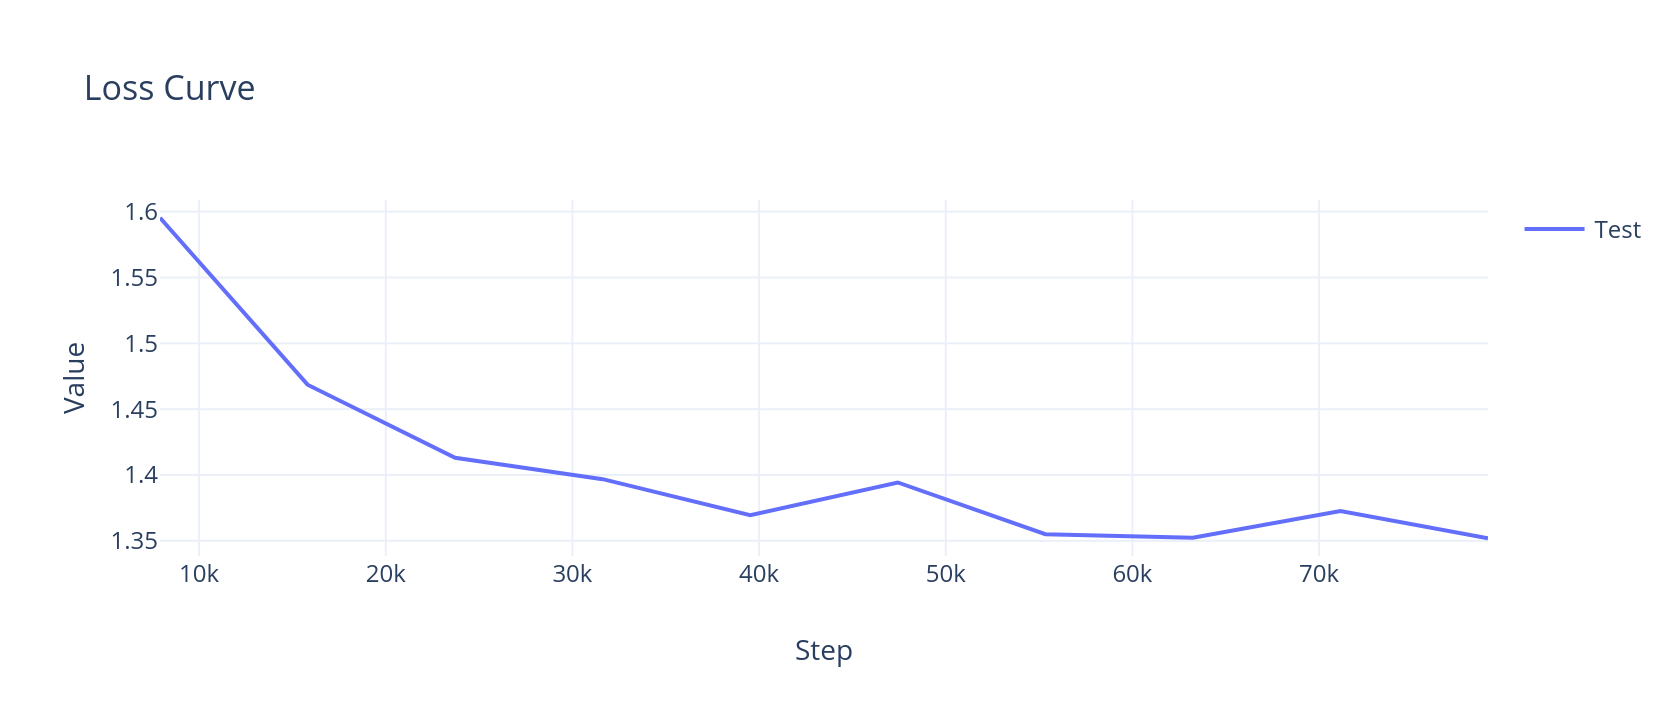
\includegraphics[width=0.5\textwidth]{images/TSCNN_loss.png}
    \caption{TSCNN Loss Curve}
    \label{fig:TSCNN_loss}
\end{figure}{}


% --------------------------------------------------------------------------------
\section{Qualitative Results}
\textbf{This section should include sample success and failure cases based on your algorithm. In presenting these examples, you can plot/display the inputs(s) in each case. Particularly: (a) find one or more examples that are correctly classified by both LMCNet and MCNet. (b) find at least one case where one input is correct while the other is incorrect. (c) find one case where late fusion outperforms individual inputs, (d) find one example where all methods fail. }

In conducting a further analysis, we found that the 5395 test samples given was reduced by averaging the logits of respective files per batch. This gave us a total of 977 samples of averaged logits spanning all batches. Out of those 977 samples, 641 were classified correctly by both LMCNet and MCNet (figure \ref{fig:LMC_MC_True}), 65 were classified correctly by LMCNet but not MCNet (figure \ref{fig:LMC_True}), 122 were classified correctly by MCNet but not LMCNet (figure \ref{fig:MC_True}), 151 were classified incorrectly for both (figure \ref{fig:LMC_MC_False}). We then used TSCNNNet, which does better overall and, unsurprisingly, doesn't do much better on the cases where both LMCNet and MCNet fail. In fact, out of the 151 samples where both LMCNet and MCNet fail, TSCNNNet only correctly classifies a single one (figure \ref{fig:LMC_MC_False_TSCNN_True}).

The figures below represent the spectograms of some of the 977 samples used. We only represent a single segment of the sample, which in practice is made up of several segments. However, we note the indices of all the segments in the sample, as a reference the test data split in the given pre-prepared dataset.


\begin{figure}[h]
    \centering
    \includegraphics[width=0.5\textwidth]{images/LMC_MC_True.png}
    \caption{Correct classification by both LMCNet and MCNet. This represents a segment of 189982-0-0-23.wav (air-conditioner). The indices of the segments making up the sample are \{3064 - 3070\}.}
    \label{fig:LMC_MC_True}
\end{figure}{}

\begin{figure}[h]
    \centering
    \includegraphics[width=0.5\textwidth]{images/LMC_True.png}
    \caption{Correct classification by LMCNet but not MCNet. This represents a segment of 115241-9-0-9.wav (street music). The indices of the segments making up the sample are \{416 - 421\}.}
    \label{fig:LMC_True}
\end{figure}{}

\begin{figure}[h]
    \centering
    \includegraphics[width=0.5\textwidth]{images/MC_True.png}
    \caption{Correct classification by MCNet but not LMCNet. This represents a segment of 93567-8-0-6.wav (siren). The indices of the segments making up the sample are \{5175 - 5181\}.}
    \label{fig:MC_True}
\end{figure}{}

\begin{figure}[h]
    \centering
    \includegraphics[width=0.5\textwidth]{images/LMC_MC_False.png}
    \caption{Incorrect classification by both LMCNet and MCNet. This represents a segment of 167464-0-0-6.wav (air-conditioner). The indices of the segments making up the sample are \{2244 - 2250\}.}
    \label{fig:LMC_MC_False}
\end{figure}{}

\begin{figure}[h]
    \centering
    \includegraphics[width=0.5\textwidth]{images/LMC_MC_False_TSCNN_True.png}
    \caption{Incorrect classification by both LMCNet and MCNet but correctly classified by TSCNNNet. This represents a segment of 77901-9-0-6.wav (street music). The indices of the segments making up the sample are \{4690 - 4696\}.}
    \label{fig:LMC_MC_False_TSCNN_True}
\end{figure}{}

% --------------------------------------------------------------------------------
\section{Improvements}
\textbf{Using the same 4-conv layer architecture, propose, implement and test one potential improvement you made to your results (i.e. do not use the 6-conv or 8-conv). Note: if you describe multiple improvements, we will give you the lower mark (rather than the higher one), so choose the one you believe in. Cover any implementation details required to understand and replicate your modifications. Report your improved results in tabular format for all metrics. Do not include any pieces of code, but you can include pseudo-codes if needed. Note: any improvements should be made using the same dataset, train/test split and evaluation metrics used earlier. Improvements can include changes to architecture, hyper-parameters and learning algorithm. Your choice should be justified theoretically and experimentally. }

Maybe use filter banks as a feature to replace LM or MFCC, will be simple to just add the code to generate filters and just do it in a similar way to other 
\href{code here}{https://www.kaggle.com/ybonde/log-spectrogram-and-mfcc-filter-bank-example}

% --------------------------------------------------------------------------------
\section{Conclusion and Future Works}
Summarise what your report contains in terms of content and achievements. 
Suggest future work that might extend, generalise or improve the results in your report. 

% --------------------------------------------------------------------------------


% \section*{References}
% Please number citations consecutively within brackets \cite{b1}. The 
% sentence punctuation follows the bracket \cite{b2}. Refer simply to the reference 
% number, as in \cite{b3}---do not use ``Ref. \cite{b3}'' or ``reference \cite{b3}'' except at 
% the beginning of a sentence: ``Reference \cite{b3} was the first $\ldots$''

% Number footnotes separately in superscripts. Place the actual footnote at 
% the bottom of the column in which it was cited. Do not put footnotes in the 
% abstract or reference list. Use letters for table footnotes.

% Unless there are six authors or more give all authors' names; do not use 
% ``et al.''. Papers that have not been published, even if they have been 
% submitted for publication, should be cited as ``unpublished'' \cite{b4}. Papers 
% that have been accepted for publication should be cited as ``in press'' \cite{b5}. 
% Capitalize only the first word in a paper title, except for proper nouns and 
% element symbols.

% For papers published in translation journals, please give the English 
% citation first, followed by the original foreign-language citation \cite{b6}.

\begin{thebibliography}{00}
\bibitem{b1} Y. Sung, K. Zhang, J Wang and K Madani. ``Environment sound classification using a two-Stream CNN based on decision-level fusion.'' In Sensors 19(7), 2019.
\bibitem{piczak}Piczak, Karol J. "Environmental sound classification with convolutional neural networks." 2015 IEEE 25th International Workshop on Machine Learning for Signal Processing (MLSP). IEEE, 2015.
\bibitem{meyer} Meyer, Matthias, Lukas Cavigelli, and Lothar Thiele. "Efficient convolutional neural network for audio event detection." arXiv preprint arXiv:1709.09888 (2017).
\bibitem{chen} Chen, Yan, et al. "Environmental sound classification with dilated convolutions." Applied Acoustics 148 (2019): 123-132.
\end{thebibliography}
\end{document}
